\chapter{Project Management}
\label{ch:project_management}

\section{Methodology}
The design and implementation of this project is expected to be experimentation based, as there are a huge number of factors to consider in the hardware design process and the final design will be based on how these factors affect performance. The hardware implementation and software tests design and implementation will be dependant on this design stage, and an agile methodology will be used to allow for changes in the objectives as the design experimentation progresses.

\section{Progress Tracking and Time Management}
Tracking progress has been completed using a Kanban Trello board, shared with the project supervisor. This board is contains all tasks on the project, sorted into various categories depending on their current state: not started, doing, blocked, completed. The board also contains extra information, such as a category for questions/issues and submission dates.

Each task on the board is colour coded and has a label that describes the type of task. Each task is also assigned a due date - this has been used to make decisions about what tasks to work on next, and makes it clear when we are failing to meet the current schedule. An example task is shown in \ref{fig:trello}, which includes a 'todo' list of what needs to be completed for the task to be checked off.

\begin{figure}[h!]
    \centering
    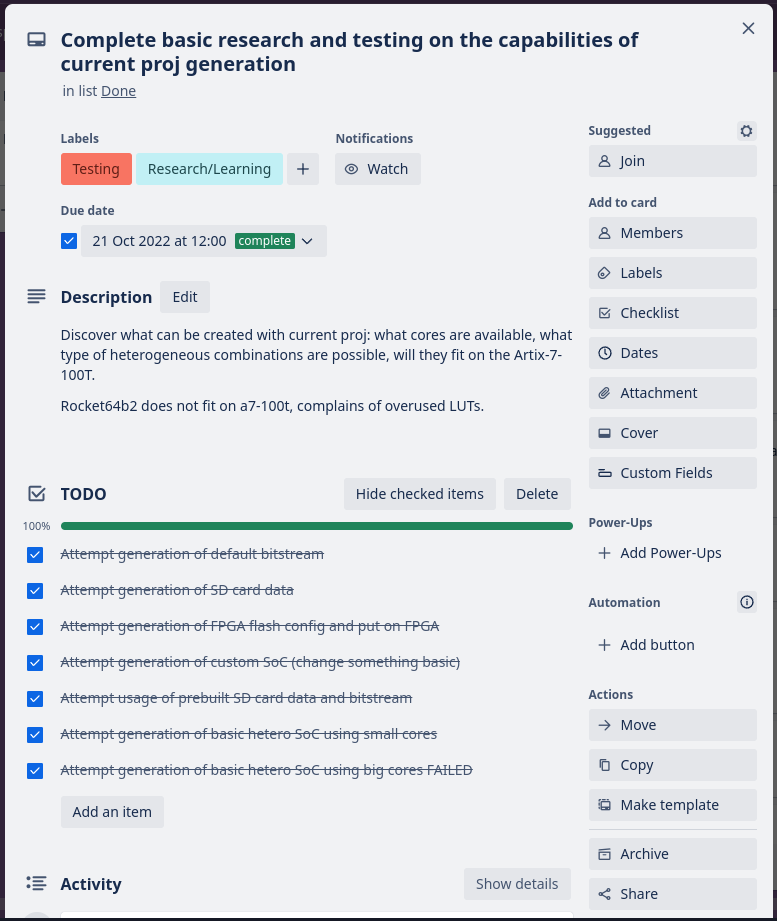
\includegraphics[width=\textwidth]{img/trello.png}
    \caption{Trello task for research into vivado-risc-v\cite{vivado-risc-v}}
    \label{fig:trello}
\end{figure}

A project diary has also been kept, detailing all work completed on the project and the dates of work. Each time work has been done on the project, we have written what was achieved, anything new that was learnt and the current thoughts on what needs to be done next time. This has meant that though there were occasions when there was over 5 days between work being done on the project, we could read the last few session notes to be reminded of the current project state and next steps.

\begin{figure}
    \centering
    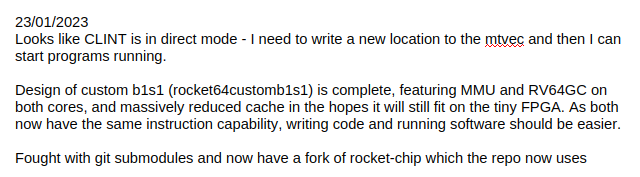
\includegraphics[width=\textwidth]{img/example_diary_entry.png}
    \caption{Example project diary entry}
    \label{fig:diary}
\end{figure}

%todo maybe gantt chart

\section{Risks} %todo maybe remove this
\begin{center}
    \begin{table}[htbp!]
        \begin{tabularx}{\textwidth}{sbbs}
            \hline
            Risk & Risk Description & Mitigation & Risk level \\
            \hline
            FPGA is too small & As the design for the SoC grows larger and more complex, it will require a greater amount of LUTs. This may result in a larger design than the FPGA to be used can implement. & This risk could be mitigated by purchasing a larger FPGA, or by reducing the complexity of the design and objectives. & High \\
            \hline
            Student is unable to work & Either by illness or other matters, the student is unable to continue work on the project for an extended period. & Mitigating this risk is difficult as illness cannot be predicted, but the likelihood of this occurring is very low. & Low \\
            \hline
            Concept is flawed/ impossible/ too difficult & As the project progresses, it appears that the main objectives of the project cannot be completed either at all, or in the time-frame provided. & The objectives and scope of the project can be changed/reduced in order to produce a full piece of work by the deadline. & Low \\
            \hline
        \end{tabularx}
    \end{table}
\end{center}